\section{Définitions}
Avant de commencer à détailler les grandes lignes de notre projet, une définition de quelques termes utilisés dans ce qui suit s'avère nécessaire.
\\

\textbf{Terminal de paiement électronique :} Le terminal de paiement électronique (TPE) est un système matériel pour le traitement des paiements par carte dans les magasins. 

%


\textbf{ProwerCard (PWC) :} PowerCARD est la suite complète de solutions de HPS qui couvre toute la chaîne de valeur des paiements en permettant des paiements innovants grâce à sa solution omni-channel qui permet le traitement de toutes les transactions en provenance de tous les canaux initiées par n'importe quel moyen de paiement.

\textbf{PowerCARD-xPOS :} La solution PowerCARD-xPOS et l'une de la suite complète de solutions de HPS. PowerCARD-xPOS peut aider les fournisseurs de paiements, les détaillants et les banques à piloter les appareils, changer d'autorisation, capturer les données de transaction et gérer la compensation et le règlement de manière rentable, dynamique et efficace, et à déployer rapidement de nouveaux services et simplement un déploiement global des appareils, tout en réduisant au minimum les coûts de maintenance et d'administration.

\textbf{Pos monitoring :} le Pos monitoring est une partie de la solution PowerCARD-xPOS qui peut aider les utilisateurs des TPE à la supervision de leurs TPE.


\begin{figure}[h!]  
  \centering
    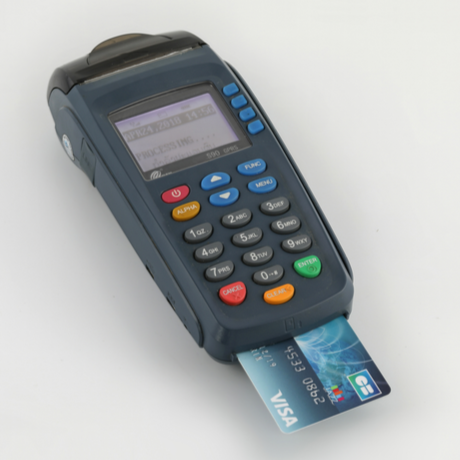
\includegraphics[width=0.9 \textwidth]{chapitre2/Figures/fdt.png}
  \caption{Exemple de terminal de paiement électronique}
\end{figure}
\newpage